\documentclass[aspectratio=169, 10pt]{beamer}
\usetheme{Madrid}
\usecolortheme{default}
\usepackage[utf8]{inputenc}
\usepackage[T1]{fontenc}
\usepackage{lmodern}
\usepackage{tikz}
\usetikzlibrary{shapes.geometric, arrows.meta, positioning}
\usepackage{booktabs}
\usepackage{listings}
\usepackage{xcolor}

\lstdefinestyle{cstyle}{
    language=C,
    basicstyle=\ttfamily\scriptsize,
    backgroundcolor=\color{black!5},
    keywordstyle=\color{blue}\bfseries,
    commentstyle=\color{green!50!black},
    stringstyle=\color{red},
    frame=single,
    breaklines=true,
}
\lstset{style=cstyle}

\title[Server HTTP Concorrente POSIX]{Progetto 1: Server HTTP Concorrente}
\subtitle{Gestione Prenotazione Aule Studio in C}
\author[Mantineo, Castorina]{Massimo Mantineo (541924) \and Pierluca Tino Castorina (545101)}
\institute[UniMe]{Università degli Studi di Messina \\ Dipartimento MIFT - Laurea in Informatica}
\date{Anno Accademico 2024/2025}

\begin{document}

\begin{frame}
    \titlepage
\end{frame}

% ==========================================
% 1. PROBLEM STATEMENT
% ==========================================
\begin{frame}{Problem Statement: Obiettivi del Progetto}
    \begin{block}{Il Problema}
        Implementare un server per la gestione di prenotazioni in grado di servire simultaneamente molteplici client, garantendo la coerenza dei dati e riducendo l'overhead computazionale di sistema.
    \end{block}
    
    \vspace{0.3cm}
    
    \textbf{Le Soluzioni Adottate:}
    \begin{itemize}
        \item \textbf{C Nativo \& POSIX:} Utilizzo delle \textit{system call} di basso livello anziché di framework moderni (Node.js, Spring) per massimizzare il controllo delle risorse.
        \item \textbf{Architettura a Thread Pool:} Sostituzione del pattern classico basato su \texttt{fork()} con un pool di worker thread pre-allocati.
        \item \textbf{Sincronizzazione Esplicita:} Impiego combinato di Semafori (per la comunicazione di rete) e Mutex (per l'accesso in mutua esclusione al database in memoria).
    \end{itemize}
\end{frame}

% ==========================================
% 2. STATO DELL'ARTE (Creata ex-novo)
% ==========================================
\begin{frame}{Stato dell'Arte: Architetture Server a Confronto}
    Per contestualizzare la scelta progettuale, è utile confrontare i principali paradigmi per la gestione della concorrenza nei server web:
    
    \vspace{0.2cm}
    \begin{itemize}
        \item \textbf{Multi-Processo:}
        Ad ogni richiesta viene associato un nuovo processo tramite \texttt{fork()}. Garantisce isolamento totale, ma presenta un elevato overhead di memoria e tempi di \textit{context switch} pesanti.
        
        \item \textbf{Modello "Thread-per-Connection":}
        Ad ogni nuova connessione accettata, il server lancia un nuovo thread dedicato tramite \texttt{pthreadCreate()}. Sebbene sia più leggero del processo \texttt{fork()}, il consumo di memoria cresce linearmente con il numero di client (ogni thread richiede il proprio stack). Inoltre, la creazione e distruzione continua di thread genera un elevato overhead, portando il sistema al collasso in caso di attacchi o carichi improvvisi.
        
        \item \textbf{Multi-Threading a Pool (Il nostro approccio):}
        Alloca un numero fisso di Thread (\textit{Worker}) all'avvio. Condivide lo stesso spazio di indirizzamento (memoria condivisa), riducendo drasticamente il consumo di RAM rispetto ai processi, delegando la gestione delle code e la mutua esclusione alle primitive POSIX (Semafori e Mutex).
    \end{itemize}
\end{frame}

% ==========================================
% 3. METODOLOGIA ED IMPLEMENTAZIONE
% ==========================================
\begin{frame}{Metodologia: Lo Stack Tecnologico}
    Il progetto è stato sviluppato e validato utilizzando esclusivamente strumenti standard e open-source:
    
    \begin{itemize}
        \item \textbf{Build System}: \texttt{Makefile} per l'automazione della compilazione.
        \item \textbf{Networking}: \texttt{Wireshark} per l'analisi dei pacchetti HTTP/TCP.
        \item \textbf{Benchmarking}: \texttt{Apache Bench (ab)} per lo stress test concorrente.
        \item \textbf{Version Control}: \texttt{Git} per la gestione del codice sorgente.
    \end{itemize}
\end{frame}

\begin{frame}{Metodologia: Architettura a Thread Pool}
    \centering
    \resizebox{0.7\textwidth}{!}{
    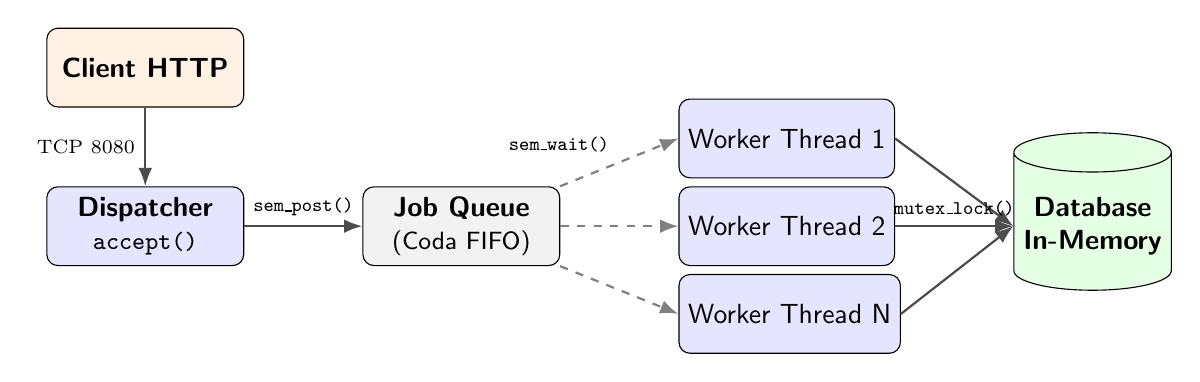
\begin{tikzpicture}[
        node distance=1.5cm and 1.5cm,
        box/.style={draw, rounded corners, minimum width=2.5cm, minimum height=1cm, align=center, fill=blue!10, font=\sffamily},
        database/.style={draw, cylinder, shape aspect=0.25, shape border rotate=90, minimum width=2cm, minimum height=2cm, align=center, fill=green!10, font=\sffamily\bfseries},
        arrow/.style={-Latex, thick, draw=black!70},
        dashed_arrow/.style={-Latex, dashed, thick, draw=black!50}
    ]

    \node[box, fill=orange!10, font=\sffamily\bfseries] (client) {Client HTTP};
    \node[box, below=1cm of client] (main) {\textbf{Dispatcher}\\ \small \texttt{accept()}};
    \node[box, right=of main, fill=gray!10] (queue) {\textbf{Job Queue} \\ \small (Coda FIFO)};
    
    \node[box, above right=0.1cm and 1.5cm of queue] (worker1) {Worker Thread 1};
    \node[box, right=1.5cm of queue] (worker2) {Worker Thread 2};
    \node[box, below right=0.1cm and 1.5cm of queue] (worker3) {Worker Thread N};
    
    \node[database, right=1.5cm of worker2] (rm) {Database\\In-Memory};

    \draw[arrow] (client) -- node[left, font=\scriptsize] {TCP 8080} (main);
    \draw[arrow] (main) -- node[above, font=\scriptsize] {\texttt{sem\_post()}} (queue);
    
    \draw[dashed_arrow] (queue) -- node[above left, font=\scriptsize] {\texttt{sem\_wait()}} (worker1.west);
    \draw[dashed_arrow] (queue) -- (worker2.west);
    \draw[dashed_arrow] (queue) -- (worker3.west);
    
    \draw[arrow] (worker1.east) -- (rm.west);
    \draw[arrow] (worker2.east) -- node[above, font=\scriptsize] {\texttt{mutex\_lock()}} (rm.west);
    \draw[arrow] (worker3.east) -- (rm.west);
    
    \end{tikzpicture}
    }
\end{frame}

\begin{frame}{Metodologia: Sincronizzazione e Flusso}
    L'utilizzo dei \textbf{Semafori} (\texttt{sem\_t}) permette di gestire la comunicazione tra thread evitando il \textit{busy-waiting} (polling attivo).
    
    \begin{itemize}
        \item \textbf{Gestione degli Stati}: Il sistema operativo pone i thread worker in \textit{Blocked State} quando la coda è vuota, azzerando il consumo di CPU.
        \item \textbf{Segnalazione (Signal/Wait)}: 
            \begin{itemize}
                \item \texttt{sem\_wait()}: Decrementa il contatore; se è zero, il thread dorme.
                \item \texttt{sem\_post()}: Incrementa il contatore e risveglia un thread dormiente.
            \end{itemize}
    \end{itemize}
\end{frame}


\begin{frame}{Implementazione: Ottimizzazioni Architetturali}
    \begin{block}{Sincronizzazione Centralizzata (Mutex)}
        L'architettura previene attivamente \textit{race conditions} e corruzione dei dati in memoria.
        L'impiego rigoroso del \textbf{Mutex} (\texttt{pthread\_mutex\_t}) garantisce che l'accesso alla memoria condivisa avvenga in totale mutua esclusione per ogni Worker Thread, assicurando l'assoluta coerenza transazionale sia in lettura che in scrittura.
    \end{block}
    
    \vspace{0.3cm}
    
    \begin{block}{De-frammentazione della Memoria Dinamica}
        La rimozione logica di una prenotazione (\texttt{DELETE}) espone al rischio di frammentazione del vettore.
        L'implementazione impiega uno \textbf{shift a sinistra} progressivo tramite un \textbf{ciclo iterativo for} all'interno dell'area protetta, garantendo la ricompattazione continua dell'array dinamico senza librerie esterne.
    \end{block}
\end{frame}



\begin{frame}[fragile]{Implementazione: Pattern Produttore-Consumatore}
    \begin{columns}
        \begin{column}{0.48\textwidth}
            \textbf{Dispatcher (Produttore)}
\begin{lstlisting}[style=cstyle]
// Accettazione e creazione job
int* client_sock = malloc(sizeof(int));
*client_sock = accept(...);

pthread_mutex_lock(&pool->queue_mutex);
// Aggiunta in coda (FIFO)
pool->queue_tail->next = job;
pool->queue_tail = job;
pthread_mutex_unlock(&pool->queue_mutex);

// Sveglia un thread worker
sem_post(&pool->queue_sem);
\end{lstlisting}
        \end{column}
        
        \begin{column}{0.48\textwidth}
            \textbf{Worker (Consumatore)}
\begin{lstlisting}[style=cstyle]
while (1) {
    // Attesa passiva (nessun busy-waiting)
    sem_wait(&pool->queue_sem);
    
    pthread_mutex_lock(&pool->queue_mutex);
    if (pool->shutdown) {
        pthread_mutex_unlock(&pool->queue_mutex);
        break; // Shutdown controllato
    }
    // Estrazione job dalla coda...
    pthread_mutex_unlock(&pool->queue_mutex);
    
    handle_client(job);
}
\end{lstlisting}
        \end{column}
    \end{columns}
\end{frame}

\begin{frame}[fragile]{Implementazione: Thread Safety sui Dati}
    L'accesso alla risorsa condivisa (il vettore delle prenotazioni) è protetto da un Mutex per garantire la coerenza dei dati durante operazioni concorrenti.
    
\begin{lstlisting}[style=cstyle]
int rm_create(resource_manager_t* rm, const char* room, ...) {
    pthread_mutex_lock(&rm->mutex); // ACQUISIZIONE LOCK
    
    if (rm->count >= MAX_RESERVATIONS) {
        pthread_mutex_unlock(&rm->mutex);
        return -1;
    }
    
    // Scrittura sicura nell'array condiviso
    strncpy(rm->reservations[rm->count].room, room, 127);
    rm->count++;
    
    pthread_mutex_unlock(&rm->mutex); // RILASCIO LOCK
    return rm->count - 1;
}
\end{lstlisting}
\end{frame}

\begin{frame}[fragile]{Implementazione: Eliminazione Atomica}
    Le operazioni logiche complesse, come la rimozione con ricompattazione (shift), devono avvenire integralmente sotto lock.
    
\begin{lstlisting}[style=cstyle]
int rm_delete(resource_manager_t* rm, int id) {
    pthread_mutex_lock(&rm->mutex); // Sezione Critica
    for (int i = 0; i < rm->count; i++) {
        if (rm->reservations[i].id == id) {
            // Shift a sinistra per ricompattare l'array
            for (int j = i; j < rm->count - 1; j++) {
                rm->reservations[j] = rm->reservations[j + 1];
            }
            rm->count--;
            pthread_mutex_unlock(&rm->mutex);
            return 0;
        }
    }
    pthread_mutex_unlock(&rm->mutex);
    return -1;
}
\end{lstlisting}
\end{frame}

\begin{frame}[fragile]{Implementazione: Shutdown Sicuro}
    La chiusura del server richiede un coordinamento per evitare \textit{deadlock} o thread rimasti in attesa sul semaforo.
    
\begin{lstlisting}[style=cstyle]
void thread_pool_destroy(thread_pool_t* pool) {
    pthread_mutex_lock(&pool->queue_mutex);
    pool->shutdown = 1; // Segnale di stop
    pthread_mutex_unlock(&pool->queue_mutex);

    // Svegliamo tutti i thread in attesa su sem_wait()
    for (int i = 0; i < pool->num_threads; i++) {
        sem_post(&pool->queue_sem);
    }

    // Join per attendere la terminazione effettiva
    for (int i = 0; i < pool->num_threads; i++) {
        pthread_join(pool->threads[i], NULL);
    }
}
\end{lstlisting}
\end{frame}

\begin{frame}{Implementazione: Specifiche API REST}
    \centering
    \renewcommand{\arraystretch}{1.2}
    \resizebox{1.0\textwidth}{!}{
    \begin{tabular}{@{}lllc@{}}
        \toprule
        \textbf{Metodo} & \textbf{Endpoint} & \textbf{Operazione nel Backend C} & \textbf{Success Code} \\
        \midrule
        \texttt{GET} & \texttt{/reservations} & Mutex Lock $\rightarrow$ Serializzazione JSON $\rightarrow$ Unlock & \texttt{200 OK} \\
        \texttt{POST} & \texttt{/reservations} & Parsing URL-Encoded, Aggiunta struct in array & \texttt{201 Created} \\
        \texttt{PUT} & \texttt{/reservations/\{id\}} & Ricerca lineare ID e aggiornamento campi & \texttt{200 OK} \\
        \texttt{DELETE} & \texttt{/reservations/\{id\}} & Memory shift a sinistra e ricompattazione array & \texttt{204 No Content} \\
        \bottomrule
    \end{tabular}
    }
\end{frame}



\begin{frame}{Implementazione: Sicurezza e Controlli}
    \textbf{Mitigazione delle criticità intrinseche in ambiente C/POSIX:}
    \begin{itemize}
        \item \textbf{Socket Leaks:} Dismissione sicura \texttt{close(fd)}.
        \item \textbf{Buffer Overflows:} Varianti sicure, errore \texttt{413}.
        \item \textbf{Interruzione SIGPIPE:} Flag \texttt{MSG\_NOSIGNAL}.
    \end{itemize}
    \centering
    \includegraphics[width=0.75\textwidth, trim=0 80 0 70, clip]{wireshark_413.png}
    \\[0.1cm]
    {\scriptsize \textbf{Figura:} Validazione Errore 413 Payload Too Large}
\end{frame}

\begin{frame}{Implementazione: Networking e Handshake TCP}
    \centering
    \includegraphics[width=0.7\textwidth, trim=0 80 0 70, clip]{wireshark_handshake.png}
    \\[0.1cm]
    {\scriptsize \textbf{Figura:} Tracciato Wireshark del Three-Way Handshake TCP.}
    
    \vspace{0.2cm}
    \begin{block}{Autenticazione}
        Le rotte sensibili richiedono l'header \texttt{Authorization: Basic} (token Base64).
    \end{block}
\end{frame}

\begin{frame}{Implementazione: Analisi Traffico HTTP}
    \begin{columns}
        \begin{column}{0.5\textwidth}
            \centering
            \includegraphics[width=1.0\textwidth, trim=0 80 0 70, clip]{wireshark_post.png}
            \\[0.1cm]
            {\tiny POST Request e Basic Auth}
        \end{column}
        \begin{column}{0.5\textwidth}
            \centering
            \includegraphics[width=1.0\textwidth, trim=0 80 0 70, clip]{wireshark_get_json.png}
            \\[0.1cm]
            {\tiny Risposta 200 OK (JSON)}
        \end{column}
    \end{columns}
\end{frame}

% ==========================================
% 4. RISULTATI
% ==========================================
\begin{frame}{Risultati: Load Testing e Performance}
    Il progetto è stato collaudato sfruttando lo strumento standard \textbf{Apache Bench (ab)}.
    La simulazione ha previsto: \textbf{10.000 richieste totali} con un livello di concorrenza di \textbf{100 client paralleli}.
    
    \vspace{0.3cm}
    
    \begin{columns}
        \begin{column}{0.5\textwidth}
            \begin{block}{Metriche di Prestazione}
                \begin{itemize}
                    \item \textbf{Total Requests:} 10.000
                    \item \textbf{Concorrenza Esterna:} 100
                    \item \textbf{Success Rate:} 100\% (0 Errori)
                    \item \textbf{Throughput:} $\sim 33.229$ Req/Sec
                \end{itemize}
            \end{block}
        \end{column}
        \begin{column}{0.5\textwidth}
            \textbf{Interpretazione Architetturale} \\
            L'assenza totale di connessioni droppate dimostra che la coda semaforica regge il carico e previene i fallimenti TCP. 
            Inoltre, il tempo di risposta mediano di appena \textbf{3.0 ms} per richiesta conferma la leggerezza dei thread worker e la corretta implementazione dei lock Mutex sulle risorse condivise.
        \end{column}
    \end{columns}
\end{frame}

% ==========================================
% 5. CONCLUSIONE E SVILUPPI FUTURI
% ==========================================
\begin{frame}{Conclusione e Sviluppi Futuri}
    L'implementazione in linguaggio C di un Thread Pool associato a socket BSD si è dimostrata una soluzione \textit{memory-safe} ad altissime prestazioni per la costruzione di architetture HTTP concorrenti.

    \vspace{0.4cm}
    \textbf{Sviluppi per Ambienti di Produzione:}
    \begin{enumerate}
        \item \textbf{Persistenza dei Dati}: Passaggio dalla struttura in RAM ad un database relazionale leggero (come \texttt{SQLite3}) per mantenere lo stato dopo il riavvio del processo.
        \item \textbf{I/O Asincrono (\texttt{epoll})}: Sostituzione delle chiamate bloccanti \texttt{read()} con un loop \textit{Event-Driven} nativo Linux per supportare il limite dei 10.000 Socket attivi.
        \item \textbf{Cifratura}: Implementazione del protocollo \textit{TLS/SSL} tramite librerie come \textit{OpenSSL} per esporre API sicure (HTTPS).
    \end{enumerate}
    
    \vspace{0.5cm}
    \centering
    \Large \textbf{Grazie per l'attenzione.}
\end{frame}

\end{document}